\section{JavaScript Semantics Specialization with Syntactic Views}\label{sec:formal}

We first define $\ires$ as a specification language to describe JavaScript
semantics.  Then, we introduce a partial evaluation in $\ires$ to reduce
JavaScript semantics using given syntactic views. We also prove its semantics
preservation.

\subsection{$\ires$: Intermediate Representations for ECMAScript}

We first introduce $\ires$, an \textbf{I}ntermediate \textbf{R}epresentations
for \textbf{E}CMA\textbf{S}cript, as a specification language for JavaScript to
describe JavaScript semantics. We define its abstract syntax, states, and
concrete semantics in the remainder of this section.

\subsubsection{Abstract Syntax}

\[
  \begin{array}{lr@{~}c@{~}c@{~}c@{~}l}
    \text{Programs} & \progset &\ni& \prog &=& (\istset, \getinst, \getnext)\\

    \text{Functions} & \funcset &\ni& \func &::=&
    \kwdef \; \kwrl \varx^* \kwrr \; \lab\\

    \text{Variables} & \varset &\ni& \varx\\

    \text{Instructions} & \instset &\ni& \inst &::=&
    \refer = \expr \mid
    \varx = \kwcl \kwcr \mid
    \varx = \expr \kwrl \expr^* \kwrr \mid \\&&&&&
    \kwif \; \expr \; \lab \; \lab \mid
    \kwret \; \expr\\

    \text{Labels} & \labset &\ni& \lab\\

    \text{Expressions} & \exprset &\ni& \expr &::=&
    \pval \mid
    \op \kwrl \expr^* \kwrr \mid
    \refer\\

    \text{References} & \referset &\ni& \refer &::=&
    \varx \mid \expr \kwsl \expr \kwsr\\
  \end{array}
\]

An $\ires$ program $\prog = (\istset, \getinst, \getnext)$ consists of initial
states and two mappings; $\getinst: \labset \rightarrow \instset$ maps labels to
their instructions, and $\getnext: \labset \rightarrow \labset$ maps labels to
their next labels, where a label $\lab \in \labset$ denotes a program point.  A
function $\func \in \funcset$ is defined with its parameters and body label.
For presentation brevity, we assume that no global or captured variables exist
in this paper.  An instruction $\inst \in \instset$ is an assignment $\refer =
\expr$, an object allocation $\varx = \kwcl \kwcr$,  a function call $\varx =
\expr \kwrl \expr^* \kwrr$, a branch $\kwif \; \expr \; \lab \; \lab$, or a
return instruction $\kwret \; \expr$.  An invocation of an abstract algorithm in
ECMAScript is compiled to a function call instruction with a new temporary
variable.  We represent loops using branch instructions with cyclic pointing of
labels in $\getnext$.  An expression is a primitive value $\pval$, an operation
$\op \kwrl \expr^* \kwrr$, or a reference $\refer$.  A reference is a variable
$\varx$ or an object field $\expr \kwsl \expr \kwsr$.  We write $\expr.\varf$ to
briefly represent $\expr \kwsl \code{"f"} \kwsr$.


\subsubsection{States}

\[
  \begin{array}{lr@{~}c@{~}l@{~}c@{~}l}
    \text{States} & \st &\in& \stset &=&
    \labset \times \ctxtset^* \times \heapset \times \envset\\

    \text{Calling Contexts} & \ctxt &\in& \ctxtset &=&
    \labset \times \envset \times \varset\\

    \text{Heaps} & \heap &\in& \heapset &=&
    \addrset \finmap \objset\\

    \text{Objects} & \obj &\in& \objset &=&
    \strset \finmap \valset\\

    \text{Environments} & \env &\in& \envset &=&
    \varset \finmap \valset\\

    \text{Values} & \val &\in& \valset &=&
    \pvalset \uplus \addrset \uplus \treeset \uplus \funcset\\

    \text{Primive Values} & \pval &\in& \pvalset &=&
    \boolset \uplus \intset \uplus \strset \uplus \cdots\\

    \text{JavaScript ASTs} & \tree &\in& \treeset\\
  \end{array}
\]

States $\stset$ consist of labels $\labset$, calling context stacks
$\ctxtset^*$, heaps $\heapset$, and environments $\envset$.  A calling context
$\ctxt \in \ctxtset$ consists of a label denoting the return point, a caller's
environment, and a return variable.  A heap $\heap \in \heapset$ is a finite
mapping from addresses to objects, and an object $\obj \in \objset$ is a finite
mappings from strings to values.  Each object allocation $\kwcl \kwcr$ creates a
unique address $\addr \in \addrset$ different from existing addresses.  An
environment $\env \in \envset$ is a finite mapping from variables to values. A
value $\val \in \valset$ is a primitive value $\pval \in \pvalset$ (e.g., a
boolean value $\bool \in \boolset$, an integer $k \in \intset$, or a string
$\str \in \strset$), an address $\addr \in \addrset$, a JavaScript AST $\tree
\in \treeset$, or a function $f \in \funcset$.

Since $\ires$ is a specification language for JavaScript, it treats JavaScript
ASTs $\treeset$ as its values. For presentation brevity, we represent a JavaScript
AST as follows:
\[
  \tree ::= \str \mid \ty_k \langle \tree^* \rangle
\]
A string $\str$ denotes a leaf node with a terminal symbol, and $\ty_k \langle
\tree^* \rangle$ denotes a non-leaf node for $k$-th alternative in the syntactic
production of nonterminal symbol $\ty$ with its subtrees $\tree^*$.  The notation
$\ty_k.\eval$ denotes an $\ires$ function for the evaluation of $k$-th
alternative in $\ty$, and it takes the AST itself and its nonterminal subtrees
as arguments. For each integer $k$, the notation $\tree[k]$ denotes $k$-th
subtree of $\tree$. If an AST $\tree$ is a subtree of another AST $\tree'$, we
represent it as $\tree \subtree \tree'$.  For example,
Figure~\ref{fig:coalesce-prod} shows a syntactic production for coalesce
expressions.  Consider the following coalesce expression:
\begin{lstlisting}[style=JS]
                    42 ?? true
\end{lstlisting}
Then, the following AST is produced as its parsing result:
\begin{figure}[H]
  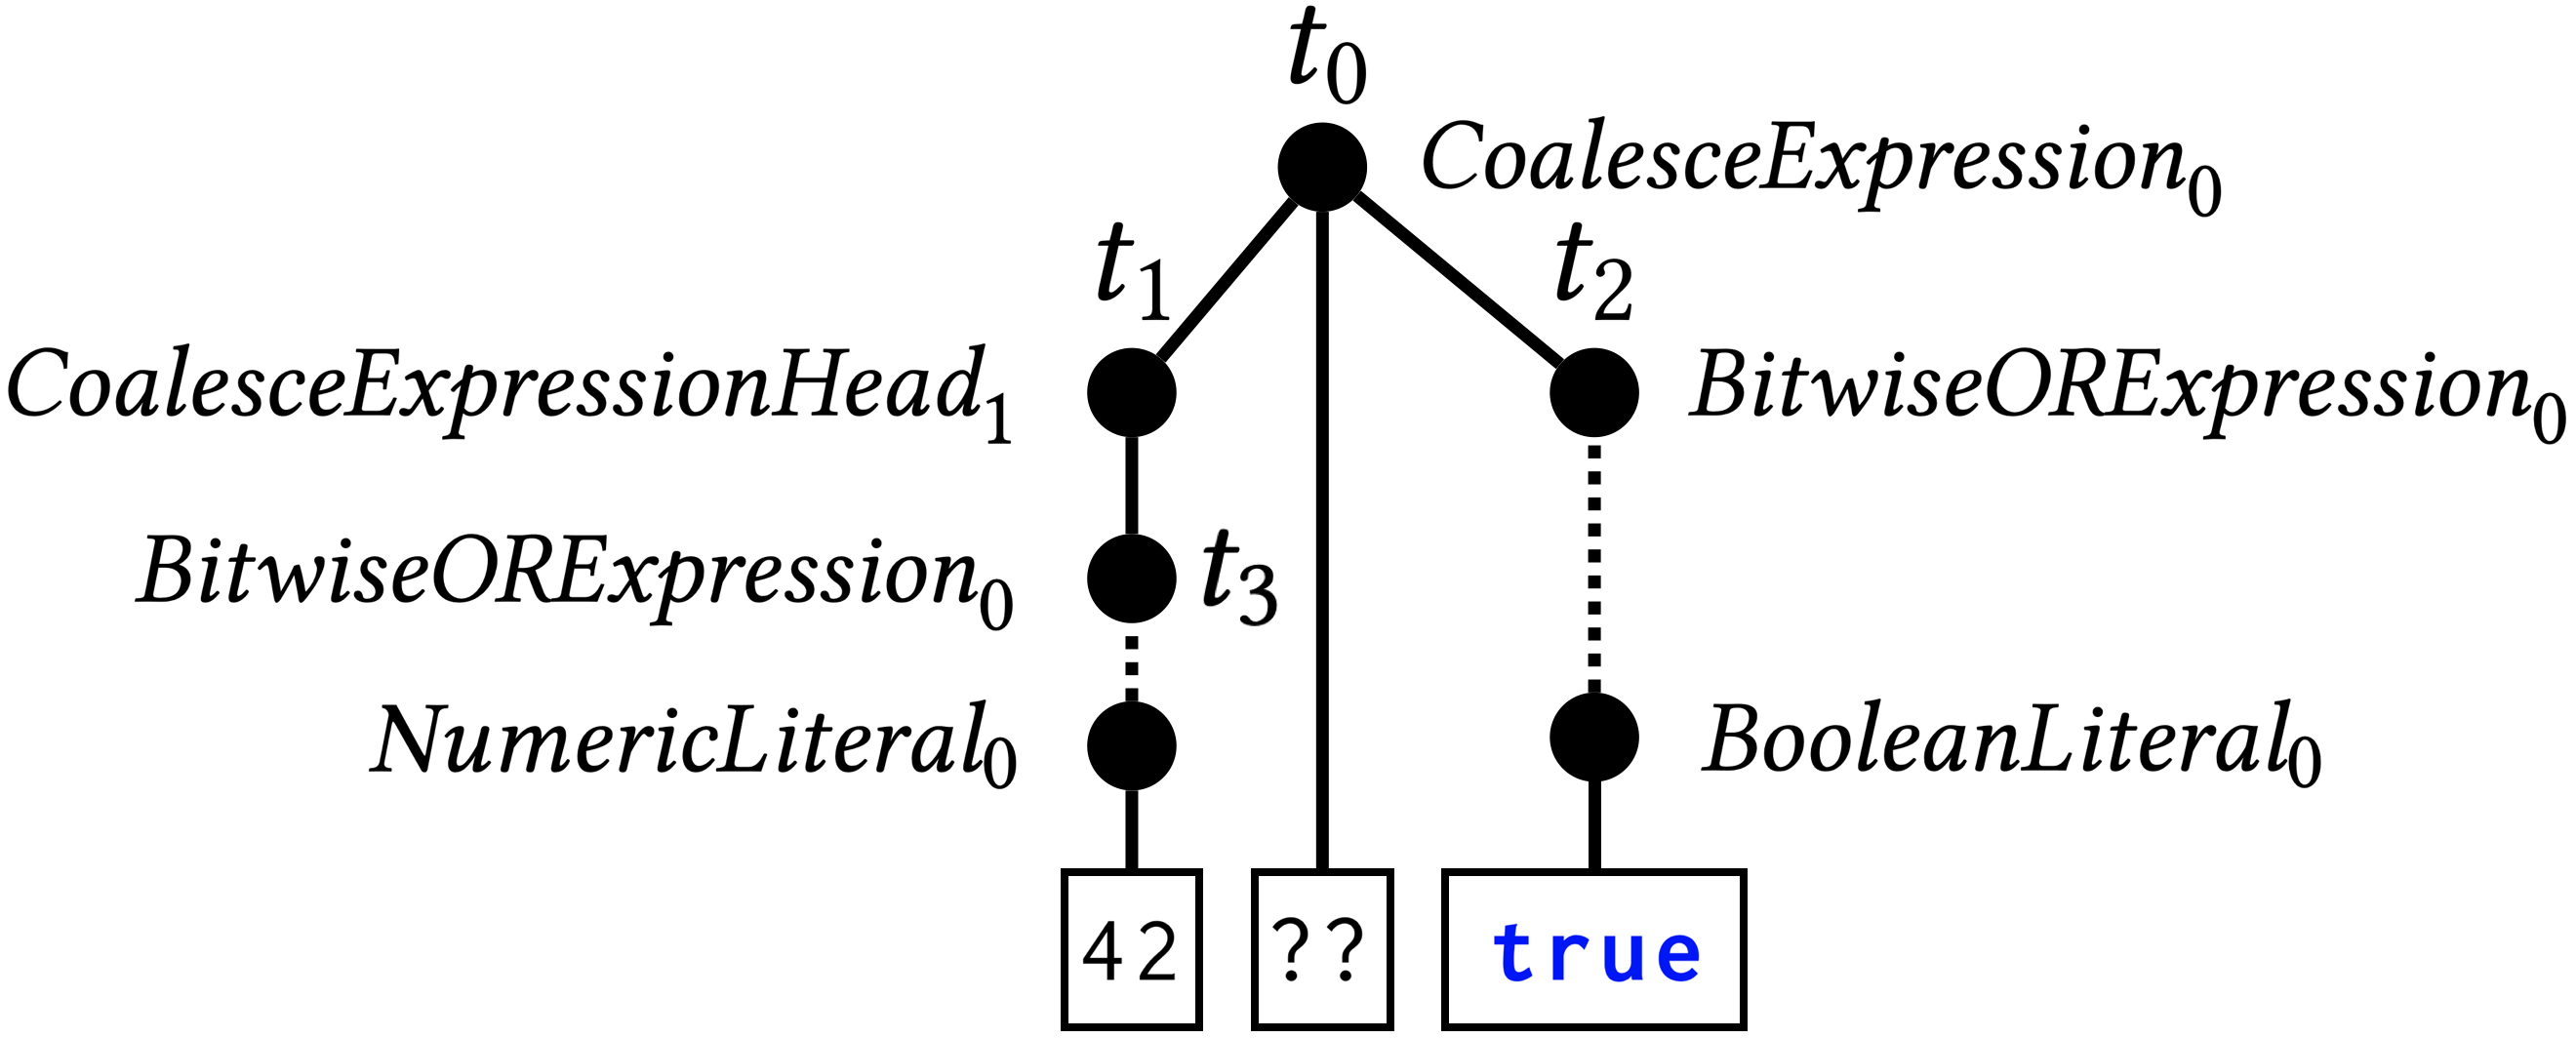
\includegraphics[width=.8\columnwidth]{img/ast-example.png}
\end{figure}
\noindent Its evaluation function $\nterm{CoalesceExpression}_0.\eval$ takes
three subtrees as arguments annotated by $\tree_0$, $\tree_1$, and $\tree_2$ in
the figure. Note that $\tree_1$ and $\tree_2$ are subtrees of $\tree_0$ (i.e.,
$\tree_1 \subtree \tree_0$ and $\tree_2 \subtree \tree_0$).


\begin{figure}
  \centering
  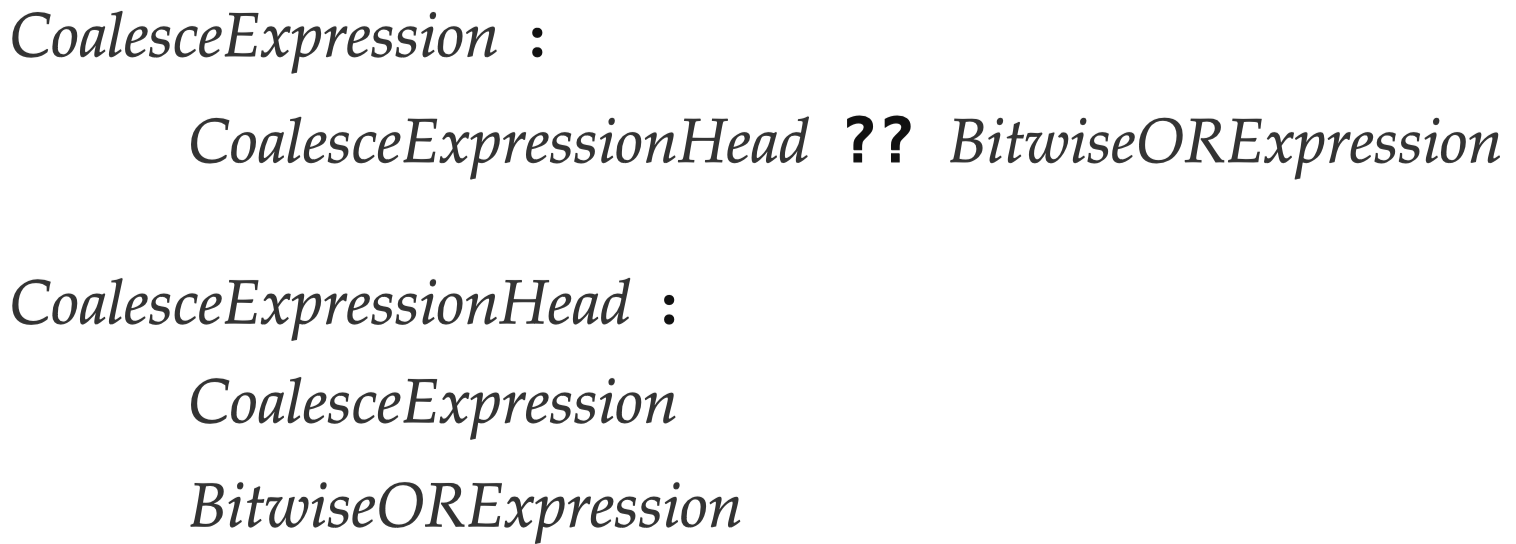
\includegraphics[width=.8\columnwidth]{img/coalesce-prod.png}
  \caption{A JavaScript syntactic production for coalesce expressions}
  \label{fig:coalesce-prod}
\end{figure}




\subsubsection{Concrete Semantics}

The concrete semantics $\sem{\prog}$ of an $\ires$ program $\prog = (\istset,
\getinst, \getnext)$ is defined as follows:
\[
  \sem{\prog} = \{ \st \in \stset \mid \ist \in \istset \wedge \ist \trans^* \st \}
\]
where $\trans^*$ denotes one or more repetition of $\trans$, and $\st \trans
\st'$ if and only if $\st = (\lab, \_, \_, \_)$ and $\sem{\getinst(\lab)}(\st) =
\st'$. Now, we define the denotational semantics of expressions, instructions,
and functions.

\paragraph{Expressions} We define the denotational semantics of expressions with
the following form:
\[
  \framebox{$\sem{\expr}: \stset \rightarrow \valset$}
\]
For each expression $\expr \in \exprset$, its semantics $\sem{\expr}$ takes a
state and returns a value as the result of expression. We define four different
cases in the semantics of expressions as
follows:
\begin{itemize}
  \item \underline{Primitive Values}:
    \[
      \sem{\pval}(\st) = \pval
    \]

  \item \underline{Operations}:
    \[
      \sem{\op \kwrl \expr_1, \cdots, \expr_n \kwrr}(\st) =
      \op(\val_1, \cdots, \val_n)
    \]
    where $\forall 1 \leq k \leq n. \; \sem{\expr_k}(\st) = \val_k$

  \item \underline{Variable Lookups}:
    \[
      \sem{\varx}(\st) = \env(\varx)
    \]
    where $\st = (\_, \_, \_, \env)$

  \item \underline{Field Lookups}:
    \[
      \sem{\expr_0 \kwsl \expr_1 \kwsr}(\st) = \val
    \]
    where
    \[
      \begin{array}{l@{~}c@{~}ll}
        \val_0 &=& \sem{\expr_0}(\st) &\wedge\\
        \val_1 &=& \sem{\expr_1}(\st) &\wedge\\
        \st &=& (\_, \_, \heap, \_) &\wedge\\
        \val &=& \left\{
          \begin{array}{ll}
            \heap(\addr)(\str)
            & \text{if} \; \val_0 = \addr \wedge \val_1 = \str\\
            \tree[k]
            & \text{if} \; \val_0 = \tree \wedge \val_1 = k\\
          \end{array}
        \right.\\
      \end{array}
    \]
\end{itemize}

\paragraph{Instructions} We define the denotational semantics of instructions
with the following form:
\[
  \framebox{$\sem{\inst}: \stset \rightarrow \stset$}
\]
For each instruction $\inst \in \instset$, its semantics $\sem{\inst}$ takes a
state and returns an updated state. We define six different cases in the
semantics of instructions as follows:

\begin{itemize}
  \item \underline{Variable Assignments}:
    \[
      \sem{\varx = \expr}(\st) =
      (\getnext(\lab), \ctxts, \heap, \env[\varx \mapsto \val])
    \]
    where $\sem{\expr}(\st) = ((\lab, \ctxts, \heap, \env), \val)$

  \item \underline{Field Assignments}:
    \[
      \sem{\expr_0 \kwsl \expr_1 \kwsr = \expr_2}(\st) =
      (\getnext(\lab), \ctxts, \heap[\addr \mapsto \obj'], \env)
    \]
    where
    \[
      \begin{array}{l@{~}c@{~}ll}
        \sem{\expr_0}(\st) &=& (\st', \addr) &\wedge\\
        \sem{\expr_1}(\st') &=& (\st'', \str) &\wedge\\
        \sem{\expr_2}(\st'') &=& ((\lab, \ctxts, \heap, \env), \val) &\wedge\\
        \obj &=& \heap(\addr) &\wedge\\
        \obj' &=& \obj[\str \mapsto \val]\\
      \end{array}
    \]

  \item \underline{Object Allocations}:
    \[
      \sem{\varx = \kwcl \kwcr}(\st) =
      (\lab, \ctxts, \heap[\addr \mapsto \epsilon], \env[\varx \mapsto
      \addr])
    \]
    where $\st = (\lab, \ctxts, \heap, \env) \wedge \addr \not\in
    \text{Domain}(\heap)$ and $\epsilon$ denotes an empty object.

  \item \underline{Function Calls}:
    \[
      \sem{\varx = \expr \kwrl \expr_1 \cdots \expr_n \kwrr}(\st) =
      (\lab_\varf, \ctxt :: \ctxts, \heap, \env')
    \]
    where
    \[
      \begin{array}{l@{~}c@{~}ll}
        \sem{\expr}(\st) &=& (\st_0, \kwdef \; \kwrl \varp_1, \cdots, \varp_n
        \kwrr \; \lab_\varf) &\wedge\\
        \sem{\expr_k}(\st_{k-1}) &=& (\st_k, \val_k) \; \forall 1 \leq k \leq n
        &\wedge\\
        \st_n &=& (\lab, \ctxts, \heap, \env) &\wedge\\
        \env' &=& [\varp_1 \mapsto \val_1, \cdots, \varp_n \mapsto \val_n]
        &\wedge\\
        \ctxt &=& (\getnext(\lab), \env, \varx)\\
      \end{array}
    \]

  \item \underline{Branches}:
    \[
      \sem{\kwif \; \expr \; \lab_\vart \; \lab_\varf}(\st) =
      \left\{
        \begin{array}{ll}
          (\lab_\vart, \ctxts, \heap, \env) & \text{if} \; \val = \true\\
          (\lab_\varf, \ctxts, \heap, \env) & \text{if} \; \val = \false\\
        \end{array}
      \right.
    \]
    where $\sem{\expr}(\st) = ((\lab, \ctxts, \heap, \env), \val)$

  \item \underline{Returns}:
    \[
      \sem{\kwret \; \expr}(\st) = (\lab, \ctxts, \heap, \env[\varx \mapsto
      \val])
    \]
    where $\sem{\expr}(\st) = ((\_, (\lab, \env, \varx) :: \ctxts, \heap, \_),
    \val)$
\end{itemize}

% \paragraph{Functions} Moreover, we define the denotational semantics of
% functions with the following form:
% \[
%   \framebox{$\sem{\func}: \heapset \times \valset^n \rightarrow \heapset \times
%   \valset$}
% \]
% For each function $\func \in \funcset$, its semantics $\sem{\func}$ takes a heap
% and values as arguments, and it returns a pair of an updated heap and a return
% value as follows:
% \[
%   \sem{\kwdef \; \kwrl \varp_1, \cdots, \varp_n \kwrr \; \lab_\varf}
%   (\heap, (\val_1, \cdots, \val_n)) = (\heap'', \val'')
% \]
% where
% \[
%   \begin{array}{l@{~}c@{~}ll}
%     \env &=& [\varp_1 \mapsto \val_1, \cdots, \varp_n \mapsto \val_n] &\wedge\\
%     \st &=& (\lab_\varf, \epsilon, \heap, \env) &\wedge\\
%     \st \trans^* \st' &=& (\lab', \epsilon, \heap', \_) &\wedge\\
%     \getinst(\lab') &=& \kwret \; \expr' &\wedge\\
%     \sem{\expr'}(\st') &=& (\st'', \val'') &\wedge\\
%     \st'' &=& (\_, \epsilon, \heap'', \_)\\
%   \end{array}
% \]





\subsection{Partial Evaluation}

We define a \textit{partial evaluation} in $\ires$ as a transformation
$\transform: \funcset \times \avalset^n \rightarrow \progset$.  It takes a
target function and abstract values $\avalset^n$ to restrict specific function
parameters with static values, then it returns the transformed $\ires$ program
in the given restriction.  We first define abstract domains of states,
environments, and values as follows:
\begin{itemize}
  \item \underline{Abstract States}: $\aelemset = \labset \rightarrow \aenvset$
    \[
      \begin{array}{lcl}
        \multicolumn{3}{l}{\elemgamma: \aelemset \rightarrow \powerset{\stset}}\\
        \elemgamma(\aelem) &=& \{ \st \in \stset \mid \st = (\lab, \_, \_, \_)
        \wedge \st \in \envgamma(\aelem(\lab)) \}\\

        \aelem \order \aelem' &\Leftrightarrow& \forall \lab \in \labset. \;
        \aelem(\lab) \order \aelem'(\lab)\\

        \aelem \join \aelem' &=& \lambda \lab \in \labset. \; \aelem(\varx) \join
        \aelem(\lab)\\
      \end{array}
    \]
  \item \underline{Abstract Environments}: $\aenvset = \varset \rightarrow
    \avalset$
    \[
      \begin{array}{lcl}
        \multicolumn{3}{l}{\envgamma: \aenvset \rightarrow \powerset{\stset}}\\
        \envgamma(\aenv) &=& \{ \st \in \stset \mid \forall \varx \in \varset.
          \; (\aenv(\varx) = \langle \val, \expr \rangle) \Rightarrow\\ &&
          \phantom{\{ \st \in \stset \mid} (\sem{\varx}(\st) = \sem{\expr}(\st) =
          \val) \}\\

        \aenv \order \env' &\Leftrightarrow& \forall \varx \in \varset. \;
        \aenv(\varx) \order \aenv'(\varx)\\

        \aenv \join \aenv' &=& \lambda \varx \in \varset. \; \aenv(\varx) \join
        \aenv(\varx)\\
      \end{array}
    \]
  \item \underline{Abstract Values}: $\avalset = (\valset \times \exprset)
    \uplus \{ \top \}$
    \[
      \begin{array}{lcl}
        \multicolumn{3}{l}{\valgamma: \avalset \rightarrow \powerset{\valset}}\\
        \valgamma(\aval) &=& \left\{
          \begin{array}{ll}
            \{ \val \} & \text{if} \; \aval = (\val, \expr) \\
            \valset & \text{if} \; \aval = \top\\
          \end{array}
        \right.\\

        \aval \order \aval' &\Leftrightarrow&
        \aval' = \top \vee \aval = \aval'\\

        \aval \join \aval' &=& \left\{
          \begin{array}{ll}
            \aval & \text{if} \; \aval = \aval'\\
            \top & \text{otherwise}\\
          \end{array}
        \right.\\
      \end{array}
    \]
\end{itemize}
An abstract state $\aelem \in \aelemset$ is a mapping from labels to abstract
environments to represent the shape of states in each label. An abstract
environment $\aenv \in \aenvset$ is a mapping from variables to abstract values
to describe values stored in variables.  An abstract value $\aval \in \avalset$
is a static value $\langle \val, \expr \rangle$ or a dynamic value $\top$.
Since non-primitive values (e.g., addresses or JavaScript ASTs) cannot be
directly represented as expressions, each static values $\langle \val, \expr
\rangle$ also keeps another way to represent itself as an expression. Now, we
define transformations of expressions and instructions, and introduce an
iterative algorithm to proceed the partial evaluation in $\ires$.

\subsubsection{Transformation of Expressions} Before defining a transformation of
expressions, we first define abstract evaluation of expressions as follows:
\[
  \framebox{$\asem{\expr}: \aenvset \rightarrow \avalset$}
\]
\begin{itemize}
  \item \underline{Primive Values}:
    \[
      \asem{\pval}(\aenv) = \langle \pval, \pval \rangle
    \]
  \item \underline{Operations}:
    \[
      \asem{\op \kwrl \expr_1, \cdots, \expr_n \kwrr}(\aenv) = \aval
    \]
    where
    \[
      \begin{array}{l@{~}c@{~}l@{~}l}
        \asem{\expr_k}(\aenv) &=& \aval_k \; \forall 1 \leq k \leq n
        &\wedge\\
        \aval &=& \left\{
          \begin{array}{ll}
            \top & \text{if} \; \exists k. \; \aval_k = \top\\
            \langle \val, \expr' \rangle & \text{if} \; \forall k. \; \aval_k =
            \langle \val_k, \expr'_k \rangle\\
          \end{array}
        \right. &\wedge\\
        \val &=& \op(\val_1, \cdots, \val_n) &\wedge\\
        \expr' &=& \op(\expr'_1, \cdots, \expr'_n)\\
      \end{array}
    \]
  \item \underline{Variable Lookups}:
    \[
      \asem{\varx}(\aenv) = \aenv(\varx)
    \]
  \item \underline{Field Lookups}:
    \[
      \asem{\expr_0 \kwsl \expr_1 \kwsr}(\aenv) = \aval
    \]
    where
    \[
      \begin{array}{l@{~}c@{~}l@{~}l}
        \asem{\expr_0}(\aenv) &=& \aval_0 &\wedge\\
        \asem{\expr_1}(\aenv) &=& \aval_1 &\wedge\\
        \aval &=& \left\{
          \begin{array}{ll}
            \langle \tree[k], \expr'_0 \kwsl \expr'_1 \kwsr \rangle & \text{if}
            \; \aval_0 = \langle \tree, \expr'_0 \rangle \wedge \aval_1 =
            \langle k, \expr'_1 \rangle\\
            \top & \text{otherwise}\\
          \end{array}
        \right.\\
      \end{array}
    \]
\end{itemize}
Then, we define the transformation of expressions as follows:
\[
  \framebox{$\transforme: \exprset \times \aenvset \rightarrow \exprset \times
  \avalset$}
\]
\[
  \transforme(\expr, \aenv) = (\expr'', \aval)
\]
where
\[
  \begin{array}{l@{~}c@{~}ll}
    \aval &=& \asem{\expr}(\aenv) &\wedge\\
    \expr'' &=& \left\{
      \begin{array}{ll}
        \pval & \text{if} \; \aval = \langle \pval, \_ \rangle\\
        \expr' & \text{if} \; \aval = \langle \_, \expr' \rangle\\
        \expr & \text{otherwise}\\
      \end{array}
    \right.\\
  \end{array}
\]

\subsubsection{Transformation of Instructions} Now, we define a transformation
of instructions using the transformation of expressions as follows:
\[
  \framebox{$\transformi: \instset \times \aenvset \rightarrow \instset \times
  \aenvset$}
\]
\begin{itemize}
  \item \underline{Variable Assignments}:
    \[
      \transformi(\varx = \expr, \aenv) =
      (\varx = \expr', \aenv[\varx \mapsto \aval])
    \]
    where
    \[
      (\expr', \aval) = \transforme(\expr, \aenv)
    \]

  \item \underline{Field Assignments}:
    \[
      \transformi(\expr_0 \kwsl \expr_1 \kwsr = \expr_2, \aenv) =
      (\expr'_0 \kwsl \expr'_1 \kwsr = \expr'_2, \aenv)
    \]
    where
    \[
      \begin{array}{l@{~}c@{~}ll}
        (\expr'_0, \_) = \transforme(\expr_0, \aenv) &\wedge\\
        (\expr'_1, \_) = \transforme(\expr_1, \aenv) &\wedge\\
        (\expr'_2, \_) = \transforme(\expr_2, \aenv)\\
      \end{array}
    \]
  \item \underline{Object Allocations}:
    \[
      \transformi(\varx = \kwcl \kwcr, \aenv) =
      (\varx = \kwcl \kwcr, \aenv[\varx \mapsto \top])
    \]

  \item \underline{Function Calls}:
    \[
      \transformi(\varx = \expr \kwrl \expr_1 \cdots \expr_n \kwrr, \aenv) =
      (\varx = \expr' \kwrl \expr'_1 \cdots \expr'_n \kwrr,
      \aenv[\varx \mapsto \top])
    \]
    where
    \[
      \begin{array}{l@{~}c@{~}ll}
        (\expr', \_) = \transforme(\expr, \aenv) &\wedge\\
        (\expr'_k, \_) = \transforme(\expr_k, \aenv) \; \forall 1 \leq k \leq
        n\\
      \end{array}
    \]

  \item \underline{Branches}:
    \[
      \transformi(\kwif \; \expr \; \lab_\vart \; \lab_\varf, \aenv) =
      (\kwif \; \expr' \; \lab_\vart \; \lab_\varf, \aenv)
    \]
    where
    \[
      (\expr', \_) = \transforme(\expr, \aenv)
    \]

  \item \underline{Returns}:
    \[
      \transformi(\kwret \; \expr, \aenv) =
      (\kwret \; \expr, \aenv)
    \]
    where
    \[
      (\expr', \_) = \transforme(\expr', \aenv)
    \]
\end{itemize}


\subsubsection{Fixpoint of Abstract Transfer Function} Finally, we define an
abstract transfer function and its fixpoint to represent abstract semantics of a
given function and abstract values:
\[
  \begin{array}{ll}
    \text{Abstract Transfer Function} & \atransfer: \aelemset \rightarrow
    \aelemset\\
\end{array}
\]

\todo


\subsection{Proof of Semantics Preservation}

\todo





\subsection{JavaScript Semantics Specialization}

This section explains how to utilize the partial evaluation for the JavaScript
semantics specialization with a user-defined syntactic view.  We first formally
define syntactic views and their operations, then we explain how to decide a
restriction of the constant propagation specialization based on a given
syntactic view.

\subsubsection{Syntatic Views} A syntatic view $\atree \in \atreeset$ is an
augmented JavaScript ASTs with abstract nodes $\top$ as follows:
\[
  \atree ::= \str \mid \ty_k \langle \atree^* \rangle \mid \top
\]
\[
  \begin{array}{lcl}
    \multicolumn{3}{l}{\treegamma: \atreeset \rightarrow \powerset{\treeset}}\\
    \treegamma(\atree) &=& \left\{
      \begin{array}{ll}
        \{ \str \} &
        \text{if} \; \atree = \str \\

        A & \text{if} \; \atree = \ty_k
        \langle \atree_1, \cdots, \atree_n \rangle \\

        \treeset & \atree = \top\\
      \end{array}
    \right.\\
    A &=& \{ \ty_k \langle \tree_1, \cdots, \tree_n \rangle \mid \forall 1 \leq
    j \leq n.  \; \tree_j \in \treegamma(\atree_j) \}
  \end{array}
\]

\subsubsection{JavaScript Program Filtering}

\[
  \atree \subtree \tree' \iff \exists \tree \in \treegamma{\atree}. \; \tree
  \subtree \tree'
\]

\todo

\subsubsection{Semantics Specialization}

\todo
